\documentclass[10pt,twocolumn]{article}
\usepackage[margin=0.8in]{geometry}
\usepackage{booktabs,graphicx,amsmath,hyperref,xcolor}
% Placeholder for text / numbers that teammates still have to fill in (search for "\todo" in this file)
\newcommand{\todo}[1]{\textcolor{red}{[TODO: #1]}}

\title{AI6102 Team Project: Predicting Survival on the Titanic}
\author{%
  LIN, YUN-FAN (G2608301F) \and LAI, WEN-TZU(G2605696C) \and WANG, YAHUI (G2606270J)\\
}
\date{}
\begin{document}
\maketitle

\begin{abstract}
We study the Kaggle \emph{Titanic -- Machine Learning from Disaster} competition, a binary classification task.
We build a preprocessing and feature-engineering pipeline, compare several learning methods with repeated
stratified cross-validation, and analyse the contribution of each feature group with an ablation study.
A regularised logistic regression reaches $\approx$0.83 CV accuracy, on par with tree ensembles.
The decision tree, SVMs and scaled $k$NN have broadly similar observed accuracies, whereas Gaussian Naive Bayes performs less well.
Adding fold-safe group-survival features raises the public score from 0.766 to 0.797.

\end{abstract}

\section{Problem Statement}
Given passenger records (class, name, sex, age, family aboard, ticket, fare, cabin, port of embarkation) predict whether a
passenger survived. The training set has 891 labelled passengers (38.4\% survived); the test set has 418 unlabelled ones.
Submissions are scored by accuracy on the hidden test labels.

\section{Challenges}
\begin{itemize}
  \item \textbf{Missing data:} Age is missing for 19.9\% of training rows, Cabin for 77.1\%, Embarked for 2 rows; the test set additionally lacks one Fare.
  \item \textbf{Small sample:} with 891 rows, CV estimates have a standard deviation of about 0.025; this variability alone does not establish whether differences between methods are statistically significant.
  \item \textbf{Mixed, messy features:} free-text names, skewed fare, categorical codes, and strongly correlated variables (Sex/Title, Pclass/Fare/Cabin).
  \item \textbf{Overfitting risk} for flexible models on few samples.
\end{itemize}

\section{Proposed Solution}
\subsection{Motivation}
EDA shows that survival depends mainly on sex (74\% female vs.\ 19\% male), class (63\%/47\%/24\%), age (58\% for children)
and family size (non-monotonic). Cabin \emph{presence} is informative (67\% vs.\ 30\%).
We therefore (i) encode these signals explicitly as features, (ii) use a regularised linear model as the main method
(Occam's razor / structural risk minimisation), and (iii) compare against non-linear alternatives to check whether extra
complexity helps.

\subsection{Exploratory Data Analysis}
Fig.~\ref{fig:eda} summarises the survival rate of the main variables on the training set. Our reading of the plots drove every later design decision:
\begin{itemize}
  \item \textbf{Sex} is the strongest signal (74.2\% female vs.\ 18.9\% male), consistent with the ``women and children first'' rule. A sex-only rule already scores 0.787 on the training set.
  \item \textbf{Pclass} (a proxy for socio-economic status) is monotone: 63.0\%, 47.3\%, 24.2\% for classes 1, 2, 3.
  \item \textbf{Age} is non-linear: 58\% survival for ages $\le12$, about 40\% for adults, 23\% above 60. A single linear age term cannot express this, so we add a child indicator.
  \item \textbf{Family size} is non-monotone: passengers with 2--4 relatives survive most, those alone or in families of five or more survive least (SibSp$\ge$5: 0\%).
  \item \textbf{Fare} is strongly right-skewed (skewness 4.79; median 14.5, maximum 512), and survival increases with fare quartile (19.7\% $\to$ 58.1\%).
  \item \textbf{Missingness is informative:} passengers with a known cabin survive 66.7\% vs.\ 30.0\% without; 79\% of the missing ages belong to third-class passengers and 76\% to passengers travelling without relatives.
  \item Classes are mildly imbalanced (38.4\% positive), so we report F1 and AUC besides accuracy and use stratified folds.
\end{itemize}
\begin{figure*}[t]\centering
  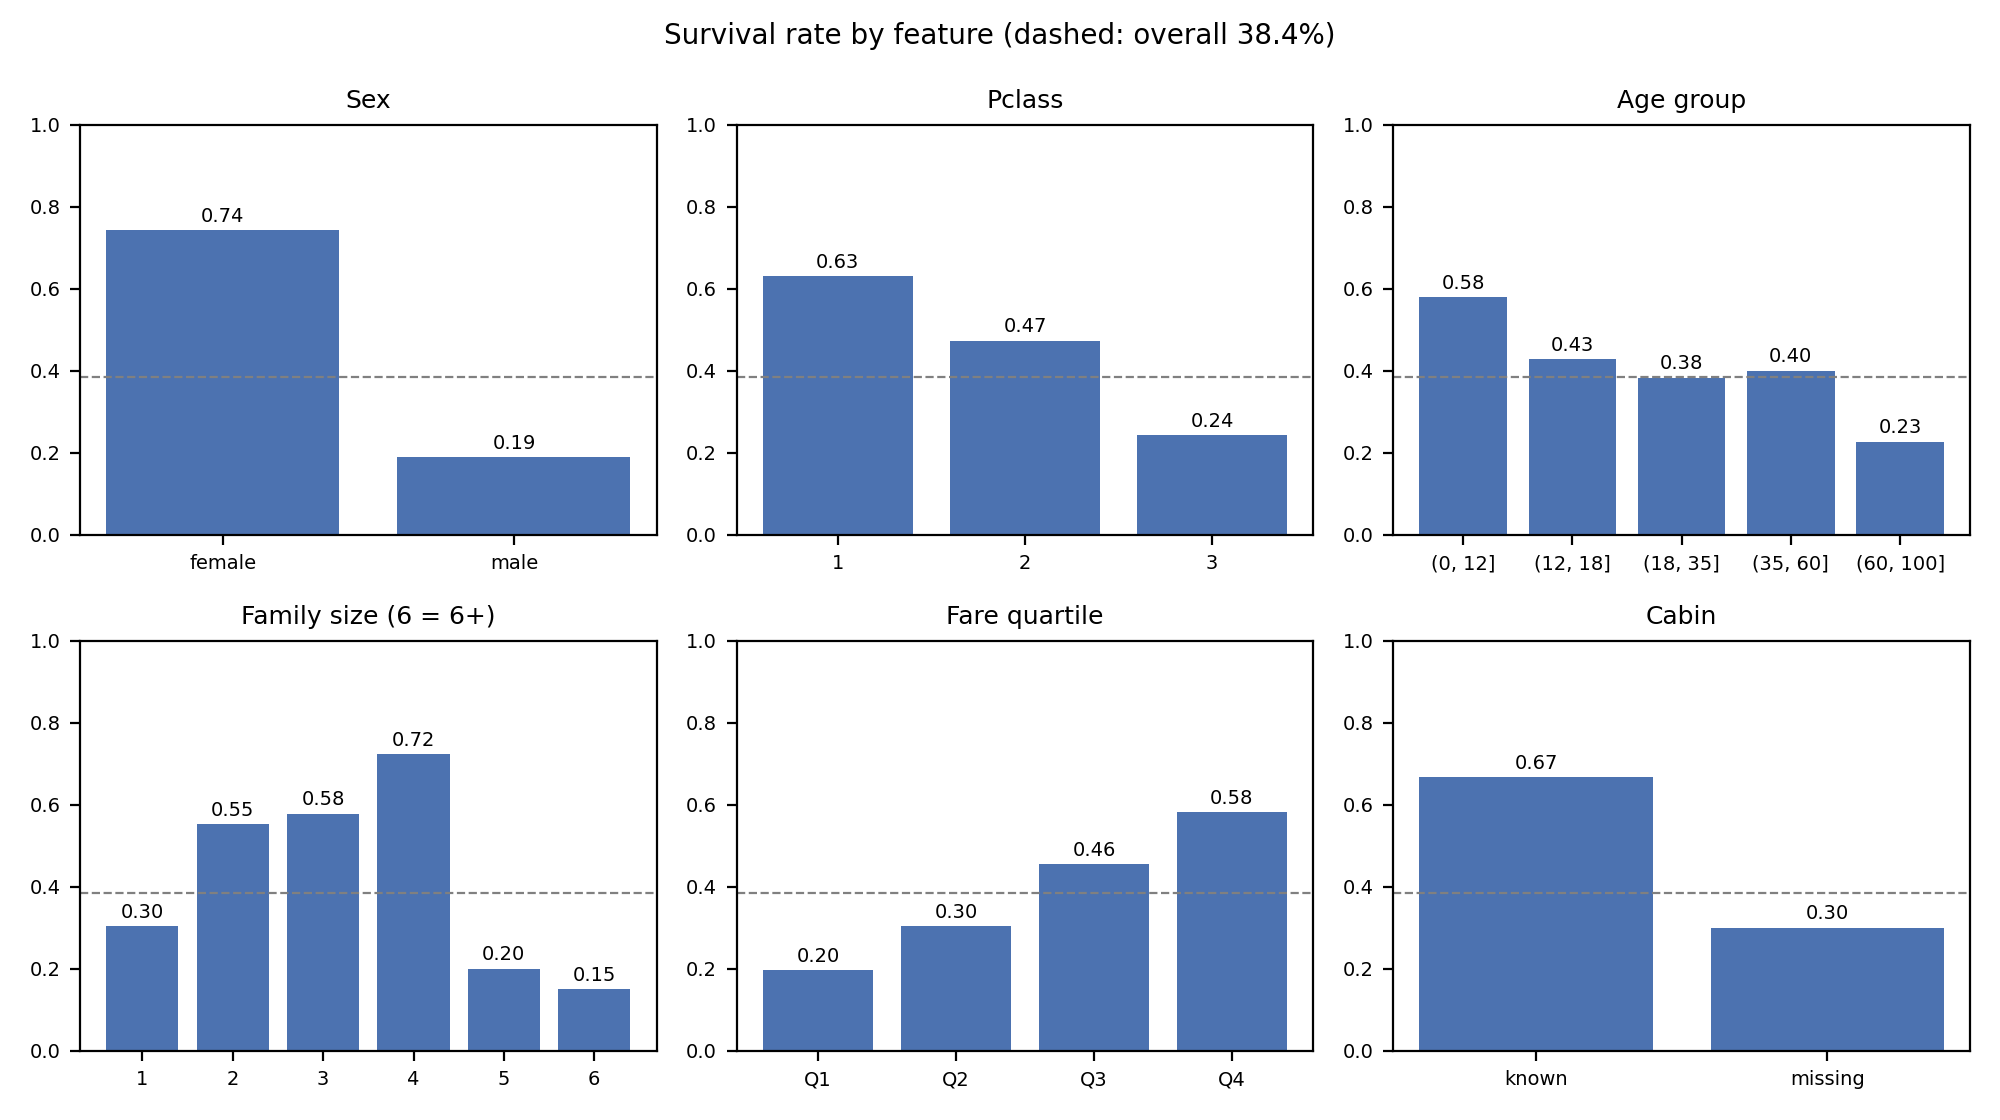
\includegraphics[width=0.85\textwidth]{figures/eda.png}
  \caption{Survival rate by feature on the training set (dashed line: overall 38.4\%).}\label{fig:eda}
\end{figure*}

\subsection{Data Preparation}
The original baseline uses training-reference imputation. For the exported dataset B used in the model comparison, however, age medians and ticket counts were computed on combined train/test covariates before CV. These features use no survival labels, but preprocessing was not refitted within folds; see the limitations below.
\begin{table}[t]
\centering\small
\caption{Missing values and how they were handled.}
\label{tab:missing}
\begin{tabular}{p{1.0cm}p{1.2cm}p{4.6cm}}
\toprule
Column & Missing (train/test) & Treatment (reason) \\
\midrule
Age & 177 / 86 & Median age of the same Title$\times$Pclass$\times$[has Parch] group; flag \texttt{AgeMissing}. Titles separate boys (Master) from men and married from unmarried women, so this is more accurate than a global median (imputation MAE 8.2 vs.\ 11.2 years). \\
Embarked & 2 / 0 & Training mode (S); only two rows. \\
Fare & 0 / 1 & Median of the passenger's class (Fare is skewed; median is robust). \\
Cabin & 687 / 327 & Not imputed: 77\% missing, so any value would be fabricated. Missingness itself is informative, so it becomes \texttt{HasCabin}. \\
\bottomrule
\end{tabular}
\end{table}
No rows were removed (only 891 samples). Columns dropped: \texttt{PassengerId} (running index), \texttt{Name} (information extracted into Title and Surname), \texttt{Cabin} (replaced by HasCabin), \texttt{Ticket} (used only as a grouping key). Categorical variables (Title, Embarked, Pclass) are one-hot encoded because they are nominal and a linear model should not assume equal spacing; numeric variables are standardised inside the model pipeline.

\subsection{Feature Engineering}\label{sec:fe}
Each feature is motivated by the EDA and validated by the ablation study (Sec.~\ref{sec:ablation}).
\begin{table*}[t]
\centering\small
\caption{Engineered features, definition and rationale.}
\label{tab:fe}
\begin{tabular}{p{2.6cm}p{6.5cm}p{7.2cm}}
\toprule
Feature & Definition & Rationale \\
\midrule
Title & Text between ``,'' and ``.'' in Name; Mlle/Ms$\to$Miss, Mme$\to$Mrs, other rare titles $\to$ Rare; one-hot. & Encodes sex, age group and marital status in one variable; also drives the age imputation. \\
Sex & female $=1$. & Strongest single signal. \\
Age, IsChild, AgeMissing & Imputed age; $\text{Age}<13$; missing indicator. & Child survival is a local effect that a linear age term cannot capture; missingness correlates with class. \\
Family flags & HasFamily ($\text{SibSp}+\text{Parch}>0$); HasChildren (adult with Parch$>0$); WithParents (minor with Parch$>0$); LargeFamily (size $\ge5$). & Survival is non-monotone in family size; flags are interpretable and removed the collinearity of SibSp, Parch and FamilySize. Without LargeFamily CV dropped by 1.7 points. \\
LogFare & $\log(1+\text{Fare})$. & Reduces skewness from 4.79 to 0.39 and raises the correlation with survival from 0.26 to 0.33; the $+1$ handles 15 free tickets. It stabilises the linear model but does not change CV accuracy. \\
HasCabin & Cabin not missing. & Proxy for deck / status. \\
TicketSize, FarePP & Passengers per ticket (counted on train+test, no labels); fare divided by ticket size. & A ticket is shared by a group, so fares are per group. \\
Group-survival rates & For every passenger: smoothed survival rate $(s+2\bar y)/(n+2)$ of the \emph{other} passengers with the same ticket / surname, their count, and the same rate restricted to women \& children and to adult men. & Relatives and travel companions tended to survive or die together. Largest single improvement (leaderboard 0.766$\to$0.797). \\
\bottomrule
\end{tabular}
\end{table*}
\paragraph{Avoiding leakage.} Group-survival features are derived from labels, so they are computed \emph{inside every CV training fold} using that fold's training labels only, with leave-one-out for the passenger's own row; test rows use all training labels. Imputation statistics and ticket counts use no labels. Scaling is fitted inside the pipeline of each fold.

\subsection{Logistic Regression}
Our main model is $L_2$-regularised logistic regression (Lectures 3--4). For a feature vector $x$,
\[
p(y{=}1\mid x)=\sigma(w^\top x+b),\qquad \sigma(z)=\frac{1}{1+e^{-z}},
\]
and the parameters minimise the regularised cross-entropy, which equals the negative log-likelihood (MLE) plus a Gaussian prior:
\[
\min_{w,b}\ \tfrac12\|w\|_2^2 + C\sum_{i}\big[-y_i\log p_i-(1-y_i)\log(1-p_i)\big].
\]
This is structural risk minimisation: $1/C$ controls model complexity (Occam's razor). The objective is convex and differentiable, so a global optimum is found with L-BFGS (liblinear for $L_1$). Features are standardised so that the penalty treats all coefficients equally. We chose logistic regression because (i) the signals found in the EDA are largely additive, (ii) with 891 samples a low-variance model is preferable, and (iii) its coefficients can be interpreted: with standardised inputs the largest were LargeFamily ($-0.60$), Female ($+0.58$), Title\_Mr ($-0.54$), Title\_Master ($+0.42$), Title\_Mrs ($+0.38$), Age ($-0.31$), HasCabin ($+0.29$) and Pclass\_3 ($-0.27$). The regularisation strength $C$ is selected by cross-validation (Sec.~\ref{sec:reg}); other models serve as comparison.

\subsection{Evaluation Protocol}
For the dataset-B comparison we use \textbf{stratified 5-fold CV repeated 5 times} (outer seed 42); some earlier feature experiments use other seeds or 10 repeats. The $k$NN, Gaussian Naive Bayes, decision tree and SVM models use nested CV: an inner stratified 5-fold splitter (shuffle enabled, seed 1) and accuracy-scored grid search within each outer training fold. The selected estimator is refitted on that outer training fold and evaluated on its held-out fold. The LR and ensemble references use the same outer splitter but fixed configurations, with separate LR parameter sweeps rather than nested selection. Metrics are accuracy (the primary selection metric), survivor-class F1 and ROC-AUC, averaged over 25 outer folds; reported standard deviations use divisor 25. For $k$NN, Gaussian Naive Bayes and the decision tree, AUC uses predicted survivor probabilities; SVM AUC uses decision scores. The Kaggle public score is used only as a final check. \textbf{Feature ablation:} we remove one feature group at a time (Sex, Pclass, Title, Age, Family, Fare, Cabin, Embarked), retrain with the same pipeline and splits, and report the change in accuracy and AUC relative to the full model; ``Only Sex'' gives the lower bound.

\textbf{Models compared.} We evaluate logistic regression ($L_2$ and $L_1$), logistic regression on PCA components, and random forest / gradient boosting as non-linear references.
We also compare scaled/unscaled $k$NN and Gaussian Naive Bayes using \texttt{team/person\_b\_knn.py} and \texttt{team/person\_b\_naive\_bayes.py}.
We further evaluate a decision tree and linear/RBF SVMs with the nested protocol in \texttt{team/person\_c\_tree\_svm.py} and \texttt{team/person\_c\_svm.py}.
All model comparisons, the regularisation sweep and the ablation use \textbf{dataset B} (23 label-free features, Sec.~\ref{sec:fe}); the group-survival features of dataset C enter only the iteration study of Sec.~\ref{sec:iter}.
For the $k$NN, Gaussian Naive Bayes, tree and SVM experiments, we drop PassengerId, Survived and fold from the predictors and use all 23 features without further feature selection.
The scaled $k$NN branch and SVM fit their scaler within each inner and outer training fold.

\section{Experiments}
\subsection{Model Comparison}
Table~\ref{tab:models} compares the methods on dataset B with repeated $5\times5$ CV and the same outer splits; tuning protocols differ as described above.
% Integration table is separate from the output overwritten by run_B_experiments.py.
% Report integration snapshot: never written by run_B_experiments.py.
% Existing reference rows copied verbatim from results_table.tex and checked
% against logistic_regression/results/results_B.csv. Decision Tree and SVM rows come from
% team/results/person_c/results_DecisionTree.csv and svm_summary.csv.
% When other members finish, update this active table as well as their sources.
\begin{table*}[t]
\centering\small
\caption{Repeated $5\times5$ stratified CV on dataset B. Accuracy is mean $\pm$ standard deviation; F1 and AUC are means. The $k$NN, Gaussian Naive Bayes, decision tree and SVM models use nested tuning, while the LR and ensemble references use fixed configurations. Nested-model parameters are selected separately in each outer fold.}
\label{tab:models}
\begin{tabular}{lccc}
\toprule
Model & Accuracy & F1 & AUC \\
\midrule
Logistic Regression (L2, $C{=}0.1$) & 0.8296 $\pm$ 0.0215 & 0.7744 & 0.8717 \\
Logistic Regression (L1, $C{=}0.3$) & 0.8298 $\pm$ 0.0223 & 0.7732 & 0.8705 \\
Logistic Regression + PCA(10) & 0.8292 $\pm$ 0.0254 & 0.7725 & 0.8707 \\
Random Forest (reference) & 0.8312 $\pm$ 0.0169 & 0.7671 & 0.8799 \\
Gradient Boosting (reference) & 0.8292 $\pm$ 0.0233 & 0.7740 & 0.8762 \\
\midrule
$k$NN (scaled, nested CV) & $0.8229\pm0.0174$ & 0.7553 & 0.8615 \\
Gaussian Naive Bayes (nested CV) & $0.7960\pm0.0305$ & 0.7441 & 0.8546 \\
Decision Tree (nested CV) & 0.8303 $\pm$ 0.0281 & 0.7714 & 0.8604 \\
SVM linear (nested CV) & 0.8274 $\pm$ 0.0259 & 0.7610 & 0.8365 \\
SVM RBF (nested CV) & 0.8240 $\pm$ 0.0202 & 0.7542 & 0.8558 \\
\bottomrule
\end{tabular}
\end{table*}

Logistic regression ($L_2$, $L_1$ and on PCA components) reaches 0.829--0.830, while the non-linear references random forest and gradient boosting reach 0.8312 and 0.8292. Their AUCs (0.8799 and 0.8762) exceed the $L_2$ LR value of 0.8717. PCA(10) gives a similar observed accuracy to LR on all 23 features; this suggests a compact representation may suffice, rather than proving that individual features are redundant.

Scaled $k$NN obtains $0.8229\pm0.0174$ accuracy, F1 0.7553 and AUC 0.8615; Gaussian Naive Bayes obtains $0.7960\pm0.0305$, F1 0.7441 and AUC 0.8546.
Their observed accuracies are below the $L_2$ LR reference (0.8296) and nested-CV decision tree (0.8303).
Scaled $k$NN has an observed AUC close to the tree's 0.8604, without establishing equivalence or superiority.
Differences in tuning protocols and overlapping CV samples limit model-only conclusions and statistical significance claims from these summaries.
The scaling comparison in Table~\ref{tab:person-b-scaling} uses the same data and split settings.

The decision tree tuned by nested CV reaches 0.8303 accuracy, linear SVM 0.8274 and RBF SVM 0.8240. The tree's rules can express interactions between sex/title, class and fare, whereas linear SVM uses an additive boundary in the engineered feature space. RBF allows local non-linear boundaries, but here has lower observed accuracy and F1 than linear SVM, despite higher AUC (0.8558 versus 0.8365). All three have lower observed AUC than the existing LR and ensemble references. These descriptive rankings do not establish statistical superiority: folds overlap and tuning protocols are not identical. The later soft-vote ensemble (LR, GB, RF) also uses target-derived group features and a different iteration protocol, so its recorded 0.840 CV accuracy and 0.79665 public score are not a controlled model-only comparison with the dataset-B tree/SVM results.

\subsection{Regularisation and Overfitting}\label{sec:reg}
Following the lecture on over-fitting and structural risk minimisation, we sweep $C$ (inverse regularisation strength) and compare training and validation accuracy (Table~\ref{tab:reg}).
\begin{table}[t]
\centering\small
\caption{Training vs.\ CV accuracy of $L_2$ logistic regression on dataset B (repeated $5\times5$ CV).}
\label{tab:reg}
\begin{tabular}{rccc}
\toprule
$C$ & Train & CV & Gap \\
\midrule
0.01 & 0.8334 & 0.8258 & 0.0076 \\
0.03 & 0.8359 & 0.8314 & 0.0045 \\
0.1 & 0.8357 & 0.8296 & 0.0061 \\
0.3 & 0.8352 & 0.8294 & 0.0058 \\
1 & 0.8355 & 0.8283 & 0.0072 \\
10 & 0.8359 & 0.8265 & 0.0094 \\
100 & 0.8358 & 0.8260 & 0.0098 \\
\bottomrule
\end{tabular}
\end{table}

For $C=0.01$ the model is slightly under-fitted (CV 0.826). For all $C\ge0.03$ the train--validation gap is below 1 point, so there is almost no over-fitting, and CV accuracy is highest at $C=0.03$ (0.831) and decreases slowly as regularisation is weakened ($C=100$: 0.826, gap 0.010), the typical onset of over-fitting. Following Occam's razor we prefer strong regularisation ($C\in[0.03,0.1]$) for equal performance. With $L_1$ regularisation only 12 (at $C=0.05$) to 14 (at $C=0.1$) of the 23 coefficients are non-zero while CV stays at 0.830--0.831, which shows that part of the feature set is redundant.

\subsection{Feature Ablation}\label{sec:ablation}
Table~\ref{tab:ablation} shows the effect of removing one feature group at a time (logistic regression, dataset B).
\begin{table}[t]
\centering\small
\caption{Feature-group ablation, logistic regression ($L_2$, $C{=}0.1$) on dataset B, repeated $5\times5$ CV.}
\label{tab:ablation}
\begin{tabular}{lcccc}
\toprule
Setting & Acc & $\Delta$Acc & AUC & $\Delta$AUC \\
\midrule
All features & 0.8296 & +0.0000 & 0.8717 & +0.0000 \\
$-$ Sex & 0.8280 & -0.0016 & 0.8711 & -0.0007 \\
$-$ Pclass & 0.8294 & -0.0002 & 0.8699 & -0.0018 \\
$-$ Title & 0.8135 & -0.0162 & 0.8632 & -0.0085 \\
$-$ Age & 0.8271 & -0.0025 & 0.8727 & +0.0009 \\
$-$ Family flags & 0.8289 & -0.0007 & 0.8688 & -0.0029 \\
$-$ Fare & 0.8319 & +0.0022 & 0.8723 & +0.0005 \\
$-$ TicketSize & 0.8296 & -0.0000 & 0.8724 & +0.0007 \\
$-$ Cabin & 0.8269 & -0.0027 & 0.8710 & -0.0008 \\
$-$ Embarked & 0.8263 & -0.0034 & 0.8721 & +0.0003 \\
Only Sex & 0.7868 & -0.0429 & 0.7669 & -0.1049 \\
\bottomrule
\end{tabular}
\end{table}

\textbf{Title} is the only group whose removal clearly hurts (accuracy $-1.6$ points, AUC $-0.009$). Removing any other single group changes accuracy by less than 0.4 points, which is within the CV standard deviation (0.02); removing Fare even raises accuracy by 0.2 points. This does not mean the other groups are unimportant: they overlap. When the family flags \emph{and} the ticket-based features (TicketSize, LogFarePP) are removed together, accuracy drops by 1.6 points (0.8132, AUC 0.8627), whereas removing either set alone costs almost nothing (0.8289 and 0.8307): the two sets describe the same ``travelling in a group'' information. Likewise Title contains Sex: removing both Title and Sex gives 0.740, but removing only Sex gives 0.828, and Sex alone gives only 0.787 (AUC 0.767). A one-at-a-time ablation therefore underestimates groups that have a substitute; group-wise removal (as done here) is more informative than removing single columns, but the conclusions must be read together with these overlaps.

\subsection{Error Analysis}
With $C=0.1$ the out-of-fold confusion matrix is TN$=477$, FP$=72$, FN$=83$, TP$=259$ (survivors: precision 0.782, recall 0.757, F1 0.770; non-survivors: recall 0.869). The model misses more survivors than it falsely flags; a lower decision threshold would trade precision for recall if detecting survivors were more important.

\subsection{Other Methods}
\subsubsection{$k$-Nearest Neighbours}

$k$NN predicts from nearby training passengers. We use Euclidean distance,
\[
 d(x,z)=\sqrt{\sum_{j=1}^{23}(x_j-z_j)^2},
\]
with exact brute-force neighbour search. Uniform voting weights neighbours equally, whereas distance voting gives closer neighbours greater influence.
The inner grid searches $k\in\{1,3,5,7,9,11,15,21,31,51\}$ and both voting schemes (20 candidates per scaling branch).
Separate unscaled and standardised pipelines use identical inner and outer splits.
Without scaling, age, fare and count variables can dominate distances to binary indicators.
Standardisation also changes the relative influence of rare binary variables, so it is a modelling choice rather than a guarantee of improvement.

\paragraph{Scaling experiment.}
Table~\ref{tab:person-b-scaling} reports held-out outer-fold results.
Standardisation raises mean accuracy from 0.7827 to 0.8229, an observed difference of 4.01 percentage points.
Each branch selects its own $k$ and voting scheme inside each outer training set: this compares tuned procedures, not a fixed-parameter scaling effect.
For a controlled diagnostic, Fig.~\ref{fig:person-b-k} fixes Euclidean distance and uniform voting and compares identical $k$ values.
At $k=15$, mean inner validation accuracy is 0.8230 with scaling and 0.7406 without it.

\paragraph{Complexity and parameter selection.}
For scaled uniform-vote $k$NN, inner training/validation accuracy is 0.9876/0.7556 at $k=1$ and 0.8422/0.8230 at $k=15$; validation accuracy falls to 0.7886 at $k=51$.
This pattern is consistent with noisy local fitting at small $k$ and excessive smoothing at large $k$.
Training accuracy at $k=1$ need not equal one when identical feature vectors or neighbour-distance ties occur.
The curves are inner-CV diagnostics, not independent held-out performance estimates.

Uniform voting is selected in 22/25 scaled outer fits (88\%); $k=7$ and $k=15$ are tied as the most frequent values (five folds each).
Three fits select distance voting with $k=51$, the grid boundary; this finite search does not establish a global optimum.
No single full-data best parameter is inferred from the frequencies.
Unscaled mean training/outer accuracy is 0.9045/0.7827, versus 0.8671/0.8229 with scaling.
Distance-weighted training scores can benefit from a training point's own zero-distance vote, so these gaps must be interpreted together with the voting settings.

\begin{table*}[t]
\centering\small
\caption{$k$NN scaling experiment on dataset B: each branch is independently tuned inside the same 25 outer folds. Outer accuracy is mean $\pm$ standard deviation; training accuracy, F1 and AUC are means.}
\label{tab:person-b-scaling}
\begin{tabular}{lcccc}
\toprule
$k$NN input & Train accuracy & Outer accuracy & F1 & AUC \\
\midrule
Unscaled & 0.9045 & $0.7827\pm0.0285$ & 0.7056 & 0.8196 \\
Standardised & 0.8671 & $0.8229\pm0.0174$ & 0.7553 & 0.8615 \\
\bottomrule
\end{tabular}
\end{table*}

\begin{figure*}[t]
\centering
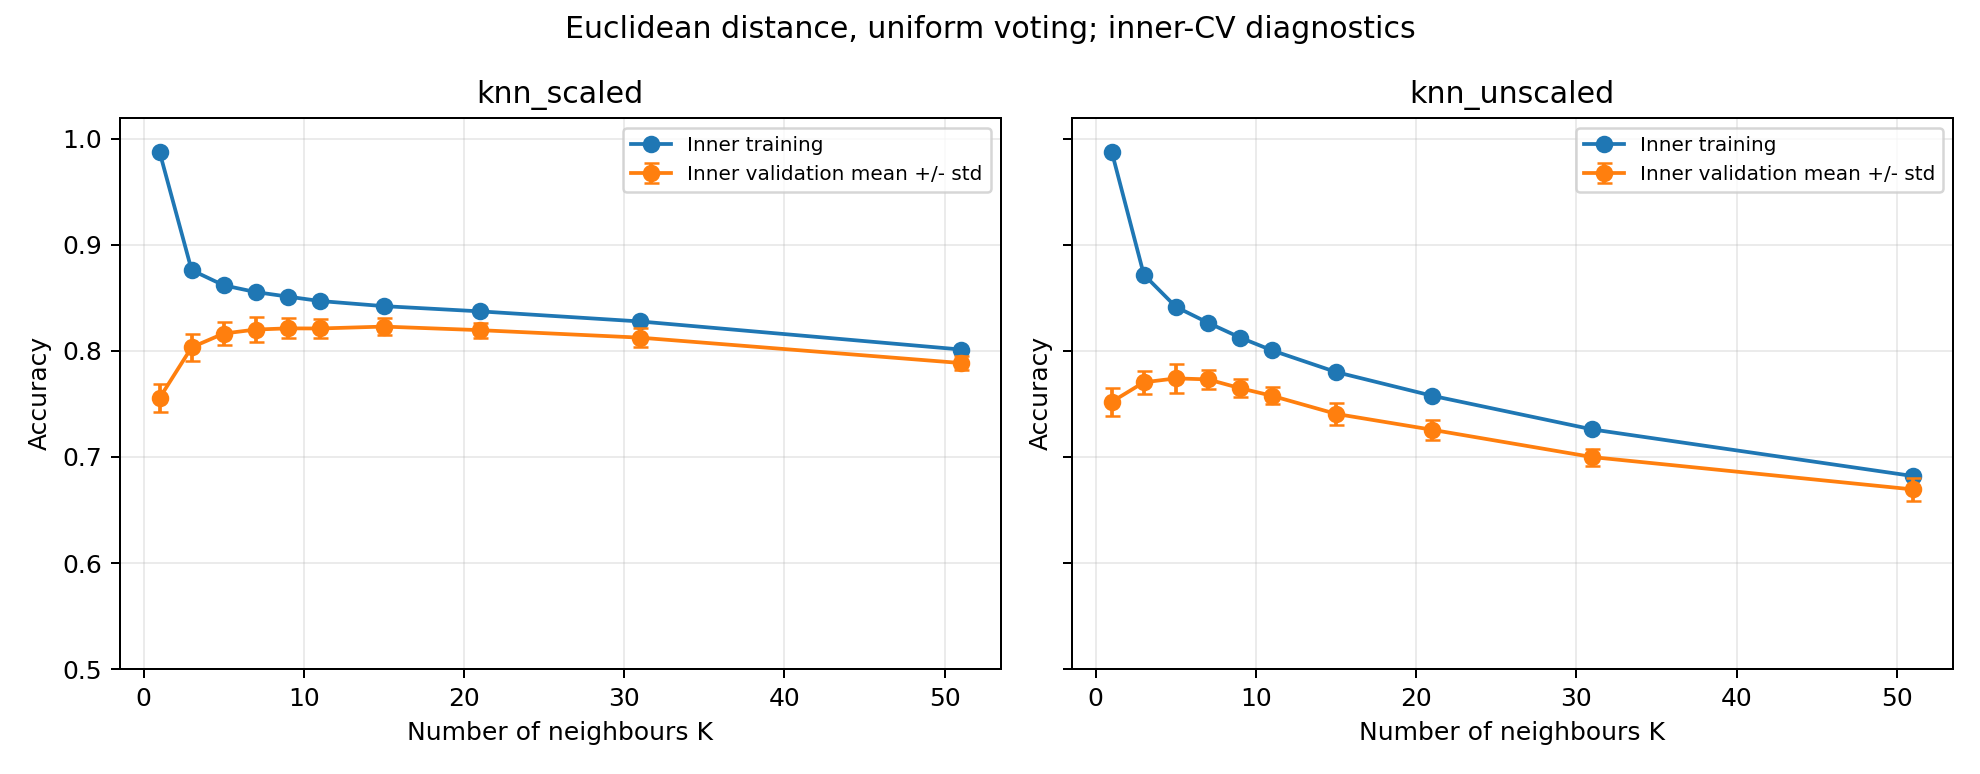
\includegraphics[width=0.95\textwidth]{figures/person_b/knn/knn_k_scaling.png}
\caption{Inner-CV $k$NN neighbour-count and scaling diagnostics, with Euclidean distance and uniform voting held fixed. Error bars show the standard deviation of inner validation means across outer training sets, not confidence intervals.}
\label{fig:person-b-k}
\end{figure*}

\subsubsection{Naive Bayes}

Gaussian Naive Bayes combines class priors with per-feature Gaussian likelihoods under conditional independence:
\[
 \hat y=\arg\max_{c\in\{0,1\}}P(y=c)\prod_{j=1}^{23}p(x_j\mid y=c).
\]
The class prior $P(y=c)$ is estimated from the class frequencies in each training split.
For feature $j$ and class $c$, Gaussian Naive Bayes estimates a mean $\hat\mu_{cj}$ and variance $\hat\sigma_{cj}^{2}$ and models the class-conditional density as
\[
 p(x_j\mid y=c)=\frac{1}{\sqrt{2\pi\hat\sigma_{cj}^{2}}}
 \exp\!\left[-\frac{(x_j-\hat\mu_{cj})^2}{2\hat\sigma_{cj}^{2}}\right].
\]
Conditional independence allows the joint likelihood to factor into these per-feature densities; Bayes' rule combines that likelihood with the class prior.
Prediction chooses the class with the larger posterior score, evaluated in log space to avoid multiplying many small numbers.

We use Gaussian Naive Bayes as a probabilistic reference model because dataset B retains continuous age and fare features.
Bernoulli Naive Bayes instead models binary indicators (0 or 1); applying it to these continuous variables would require explicit binarisation choices and would discard their original numerical detail.
We do not evaluate Bernoulli Naive Bayes here, so no claim is made that Gaussian Naive Bayes outperforms it.
Gaussian likelihoods remain only an approximation for B's one-hot and binary indicators.

\paragraph{Smoothing experiment.}
The inner grid searches \texttt{var\_smoothing} over $10^{-12},10^{-11},\ldots,10^0$ (13 candidates).
To avoid near-zero estimated variances, Gaussian Naive Bayes adds the same stability term to each class-feature variance:
\[
 \epsilon=\texttt{var\_smoothing}\cdot\max_j\operatorname{Var}_{\rm train}(X_j),
 \qquad \tilde\sigma_{cj}^{2}=\hat\sigma_{cj}^{2}+\epsilon.
\]
The smoothed variance is used in the likelihood calculation.
We use unscaled B features; rescaling would also change the smoothing effect.
Parameters are selected independently in each outer training set using inner accuracy only.

Outer accuracy is $0.7960\pm0.0305$, F1 0.7441 and AUC 0.8546, with mean training accuracy 0.8086.
The value $10^{-4}$ is selected in 16/25 folds (64\%).
Fig.~\ref{fig:person-b-nb} shows mean inner validation accuracy 0.7929 at $10^{-4}$, decreasing to 0.6158 and 0.6162 at $10^{-1}$ and $1$.
These values approach the majority-class baseline (61.6\%), consistent with excessive smoothing reducing discrimination.
Two fits select the smallest grid value ($10^{-12}$); several small values have equal inner scores, so a unique numerical optimum is not established.

\paragraph{Conditional independence and limitations.}
Conditional independence means that, after the survival class is given, one feature supplies no further information about another feature.
Sex and Title encode overlapping information; class, fare and cabin presence, and family flags and ticket size, may also retain dependencies within a class.
The one-hot indicators of a categorical variable are mutually exclusive and are not independent when multiple categories occur within a class.
These structural considerations make the independence assumption restrictive, while Gaussian likelihoods are also an approximation for binary inputs.
We have not isolated these factors with a correlated-feature-removal experiment, so they are possible limitations rather than established causes of the lower accuracy.
A marginal correlation matrix alone would not test the full conditional-independence assumption.

\begin{figure}[t]
\centering
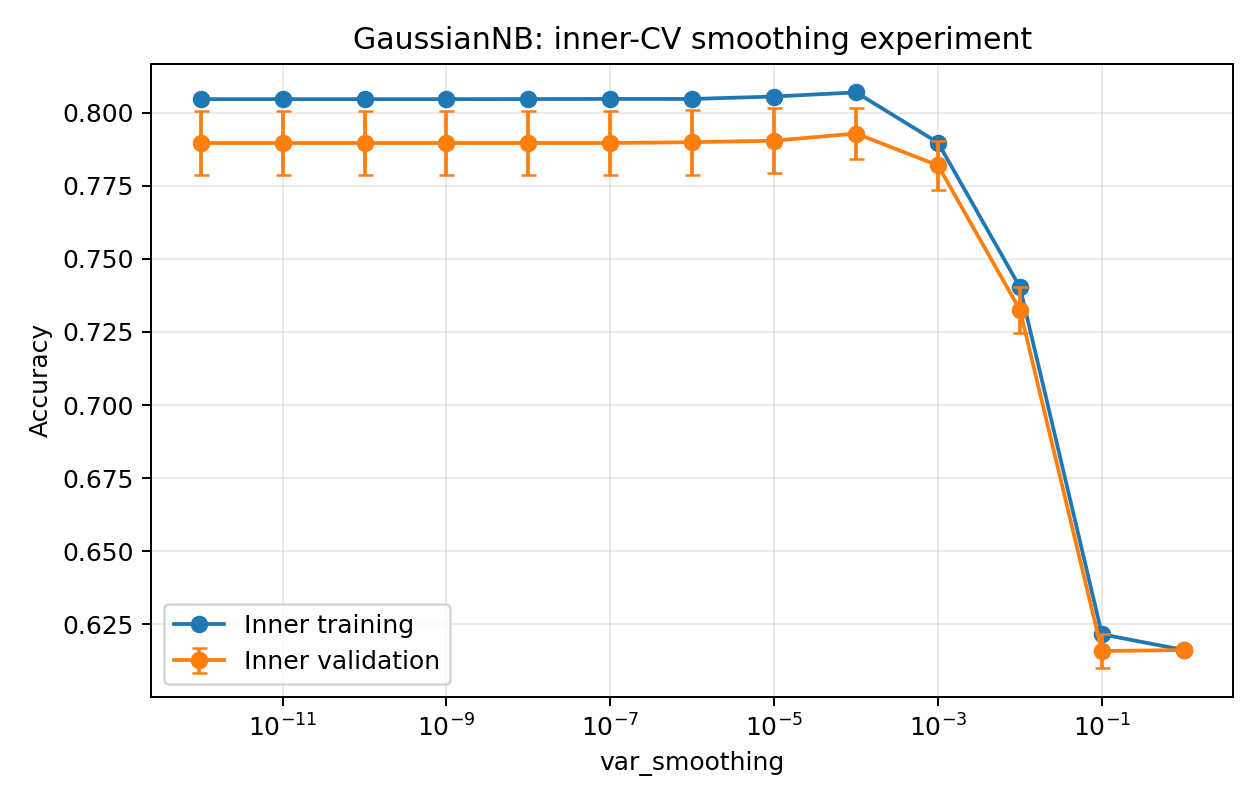
\includegraphics[width=\linewidth]{figures/person_b/naive_bayes/nb_smoothing.png}
\caption{Gaussian Naive Bayes inner-CV smoothing experiment. Error bars describe variation of inner validation means across outer training sets; outer-fold metrics appear in Table~\ref{tab:models}.}
\label{fig:person-b-nb}
\end{figure}

\subsubsection{Decision Tree}
A binary decision tree chooses feature thresholds to reduce the weighted impurity of its child nodes. At a node with class proportions $p_k$, the Gini index is
\[
G=1-\sum_{k\in\{0,1\}}p_k^2.
\]
Pure nodes have $G=0$. We use \texttt{criterion="gini"} and \texttt{random\_state=0}. The maximum depth limits successive splits, while \texttt{min\_samples\_leaf} prevents leaves supported by too few passengers. The inner grid searches depths $\{2,3,4,5,6,8,\mathrm{None}\}$ and leaf sizes $\{1,5,10,20\}$ (28 combinations); None removes the depth limit. Scaling is unnecessary for these threshold splits.

Across the 25 outer folds, accuracy is $0.8303\pm0.0281$, F1 is 0.7714, ROC-AUC is 0.8604 and training accuracy is 0.8652. The mean train--test accuracy gap is 0.0349. The most frequent selected pair is depth 4 with leaf size 1 (7/25 folds); parameters are selected separately in each fold, so this is not a single final full-data fit.

Fig.~\ref{fig:person-c-depth} shows inner-CV training and validation accuracy. At each depth, leaf size is selected independently using that outer fold's inner validation scores, then the inner means are averaged over outer folds. Depth 2 gives training/validation accuracies 0.8033/0.7886, consistent with underfitting relative to depths 4--6. At depth 6 these are 0.8779/0.8257; validation accuracy falls to 0.8208 at depth 8 and 0.8189 without a depth limit. This pattern supports controlling complexity. Since leaf size is reselected at each depth, training accuracy need not increase monotonically. These tuning diagnostics are not independent outer-test performance estimates.
\begin{figure}[t]\centering
  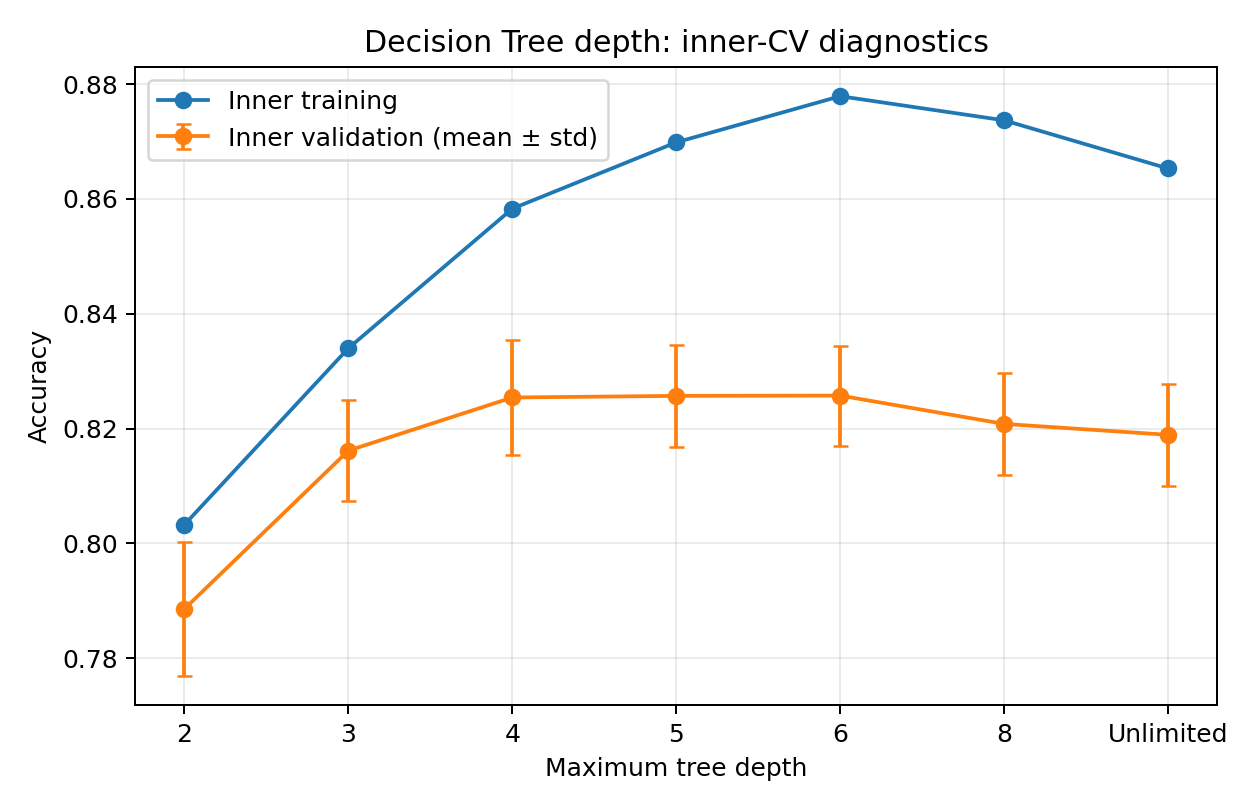
\includegraphics[width=\linewidth]{figures/person_c_tree_depth.png}
  \caption{Tree depth experiment: inner-CV training and validation means. Error bars show the standard deviation of the inner validation means across outer folds.}\label{fig:person-c-depth}
\end{figure}

Fig.~\ref{fig:person-c-importance} averages impurity-based feature importance over the 25 selected outer models. The largest mean contributions are Title\_Mr (0.4070), Female (0.1262), Pclass\_3 (0.1006), LogFarePP (0.0957) and TicketSize (0.0568). Correlated predictors such as sex and title can substitute for one another, and impurity importance can favour continuous or high-cardinality features; these values describe the fitted trees, not causal effects or a validated feature-selection rule.
\begin{figure}[t]\centering
  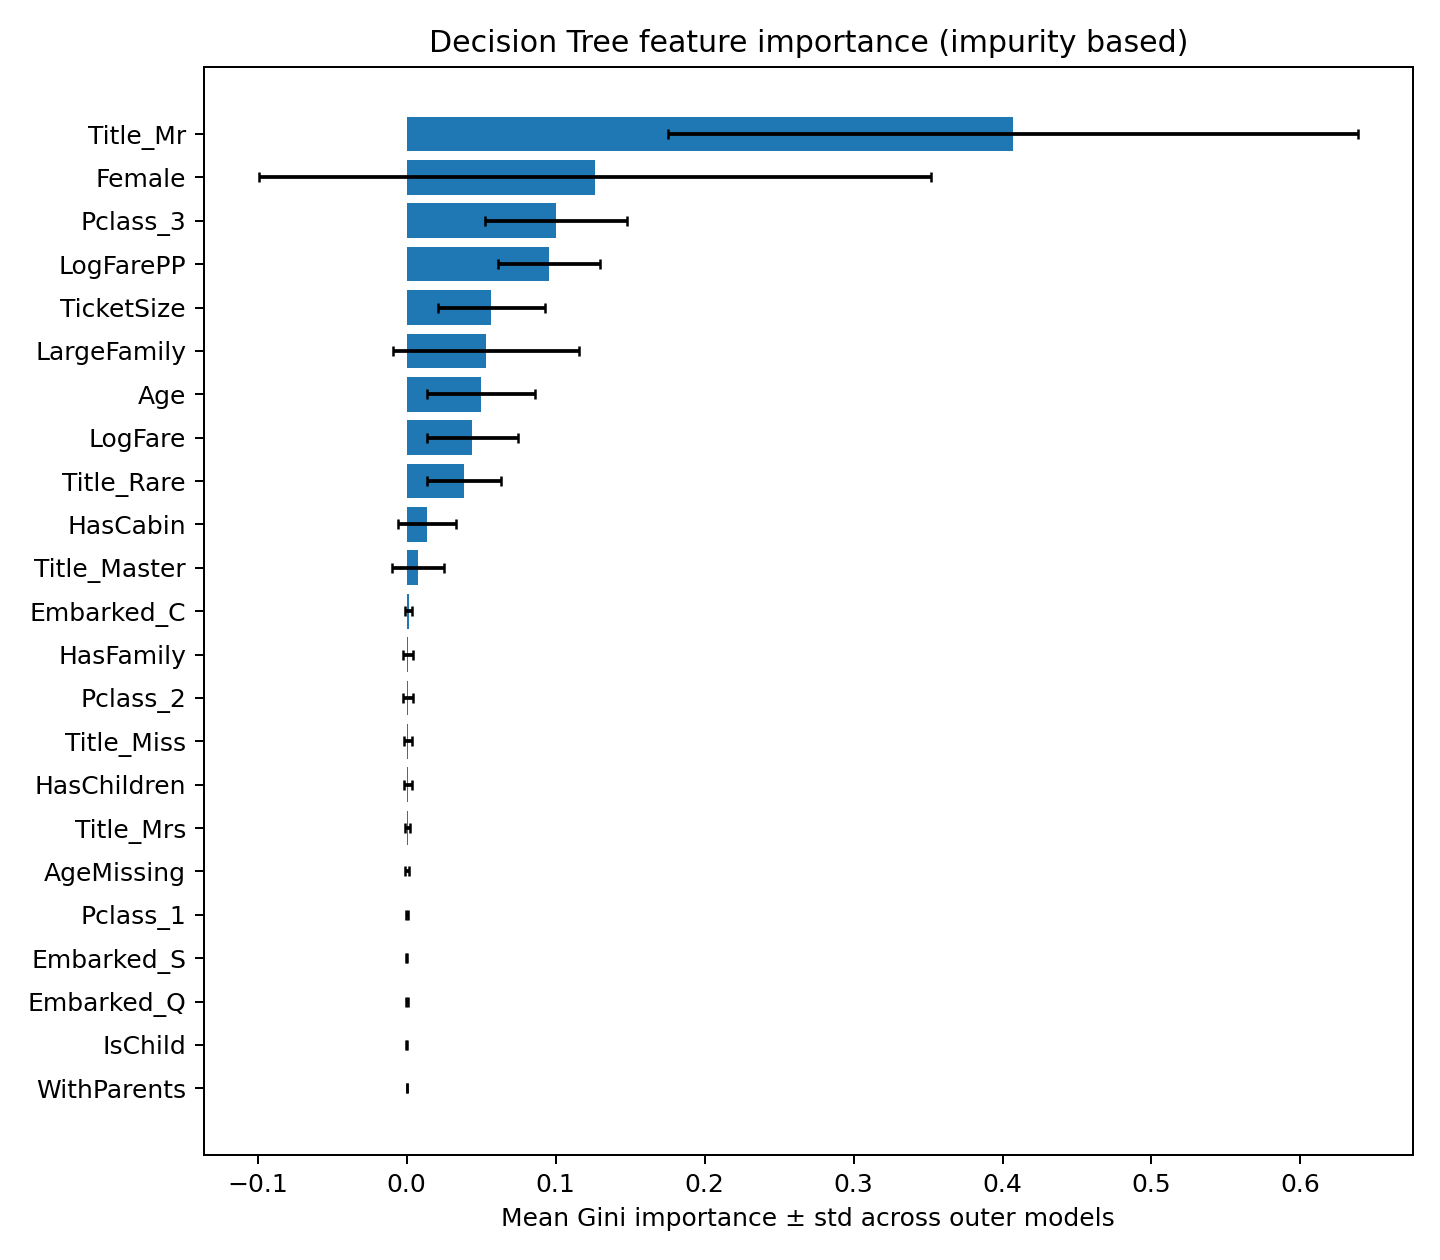
\includegraphics[width=\linewidth]{figures/person_c_tree_importance.png}
  \caption{Mean Gini importance and standard deviation across the 25 selected outer-fold trees. Symmetric error bars may extend below zero although each fitted importance is non-negative.}\label{fig:person-c-importance}
\end{figure}
\subsubsection{Support Vector Machine}
SVM balances a large margin against hinge-loss penalties for margin violations. Smaller $C$ strengthens regularisation; larger $C$ penalises violations more heavily. The linear kernel $K(x,z)=x^\top z$ yields a linear boundary in the engineered features. The RBF kernel
\[
K(x,z)=\exp(-\gamma\|x-z\|^2)
\]
allows non-linear boundaries; larger $\gamma$ makes similarity more local. Unlike logistic regression's cross-entropy objective, SVM optimises a margin-based objective and its decision scores are not calibrated survival probabilities.

Both kernels use \texttt{StandardScaler} inside the searched pipeline, fitted only to the relevant inner/outer training samples. Linear SVM searches $C\in\{0.01,0.03,0.1,0.3,1,3,10,100\}$. RBF searches $C\in\{0.03,0.1,0.3,1,3,10,100\}$ and $\gamma\in\{\mathrm{scale},0.001,0.01,0.03,0.1\}$ (35 combinations). The scale option computes $\gamma=1/(d\,\mathrm{Var}(X))$ from the scaled training matrix with $d=23$. Grid search selects by inner accuracy, not outer AUC. We use \texttt{SVC} with shrinking disabled to avoid a severe solver slowdown, tolerance 0.001, and no probability calibration; ROC-AUC is calculated from \texttt{decision\_function}.

Linear SVM obtains accuracy $0.8274\pm0.0259$, F1 0.7610, AUC 0.8365 and training accuracy 0.8280. RBF obtains $0.8240\pm0.0202$, F1 0.7542, AUC 0.8558 and training accuracy 0.8435 (Fig.~\ref{fig:person-c-kernels}). Their mean train--test gaps are 0.0006 and 0.0195. Linear $C=0.3$ is selected in 17/25 folds, and $C=0.01$ and 0.1 each in four. The most frequent RBF pair is $C=0.3$, $\gamma=\mathrm{scale}$ (6/25 folds); the remaining folds select other pairs, so no universal best pair is inferred.
\begin{figure*}[t]\centering
  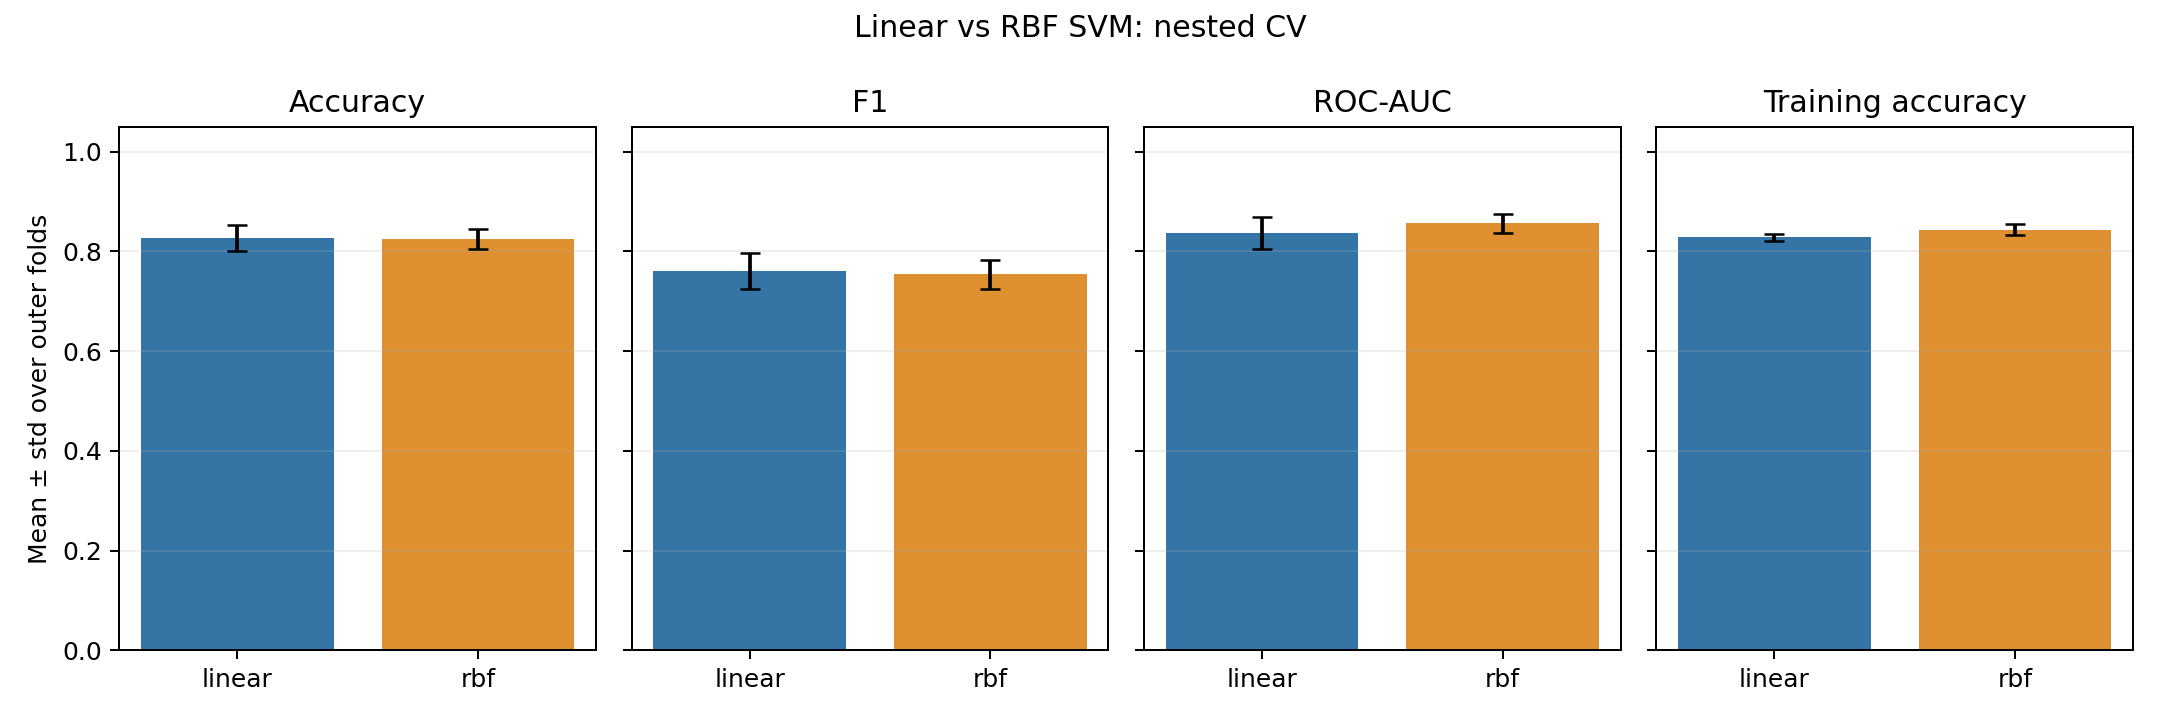
\includegraphics[width=\textwidth]{figures/svm_kernel_comparison.png}
  \caption{Nested-CV Linear/RBF SVM comparison. Bars are means and error bars are standard deviations over 25 outer folds, not confidence intervals.}\label{fig:person-c-kernels}
\end{figure*}

Fig.~\ref{fig:person-c-linear-c} shows that the mean inner validation accuracy rises from 0.8249 at $C=0.01$ to 0.8277 at $C=0.3$, then remains at the same reported value through $C=100$. The small training--validation gap does not suggest substantial overfitting in this linear grid. The RBF heatmap (Fig.~\ref{fig:person-c-rbf-grid}) shows sensitivity to both parameters: for example, $C=0.03$, $\gamma=0.001$ gives inner validation accuracy 0.616, while $C=0.3$, $\gamma=\mathrm{scale}$ gives approximately 0.831. These are tuning diagnostics averaged across outer training sets, not additional held-out performance estimates. RBF's higher AUC but lower accuracy than linear SVM indicates better observed ranking without better classification at the default decision threshold.
\begin{figure}[t]\centering
  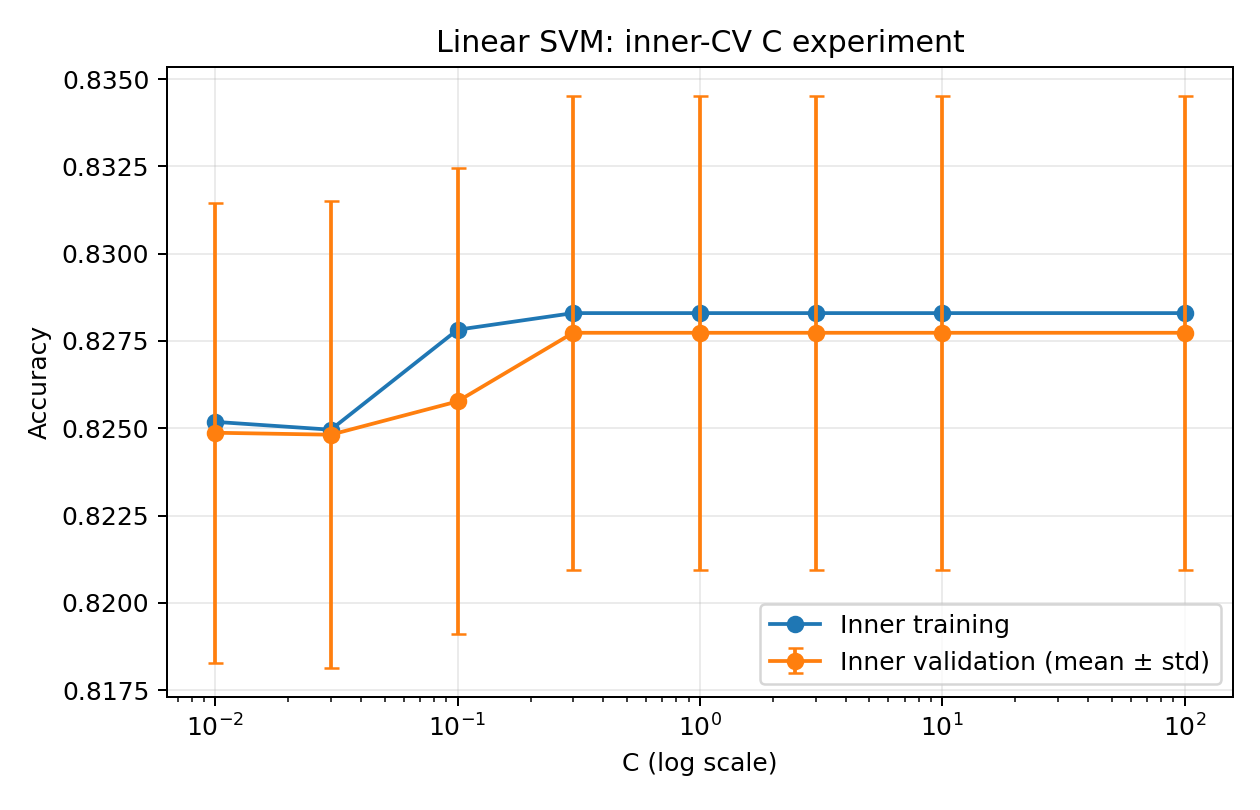
\includegraphics[width=\linewidth]{figures/svm_linear_c.png}
  \caption{Linear SVM $C$ experiment using inner-CV scores. Error bars show variation of inner validation means across outer folds.}\label{fig:person-c-linear-c}
\end{figure}
\begin{figure}[t]\centering
  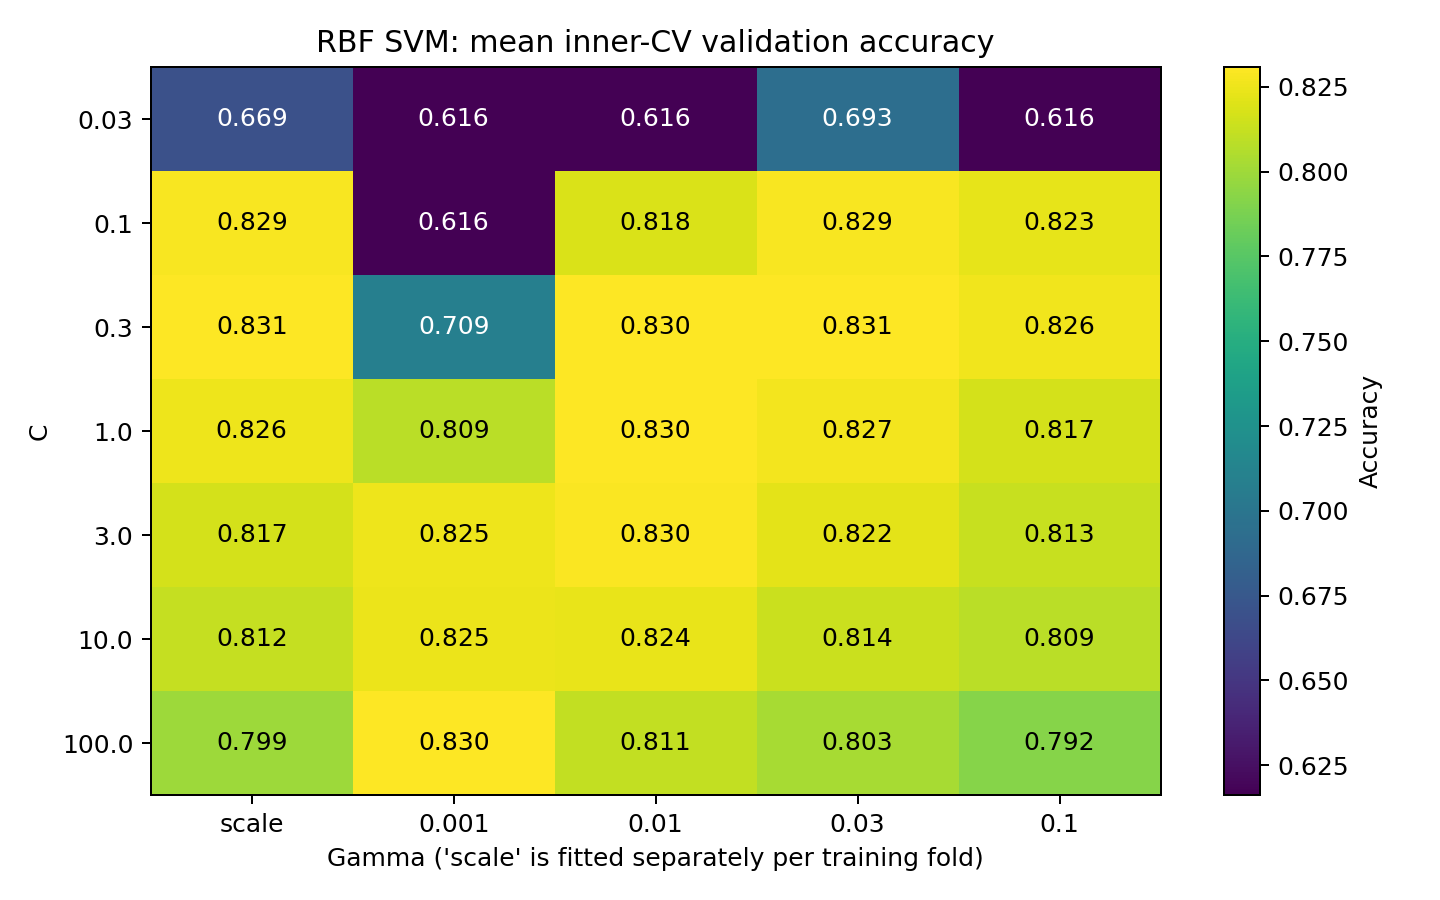
\includegraphics[width=\linewidth]{figures/svm_rbf_c_gamma_heatmap.png}
  \caption{Mean RBF inner validation accuracy over outer folds, for each $C$ and $\gamma$.}\label{fig:person-c-rbf-grid}
\end{figure}

\subsection{Iterative Improvement and Leaderboard}\label{sec:iter}
We iterated on features and models, always selecting with repeated stratified CV (identical folds for all candidates)
and recording the public leaderboard score of each submission (Table~\ref{tab:versions}).
\begin{table}[t]
\centering
\caption{Versions, CV accuracy (repeated stratified CV) and Kaggle public score (418 test passengers; one passenger $\approx 0.24$ points).}
\label{tab:versions}
\small
\begin{tabular}{p{3.9cm}cc}
\toprule
Version & CV acc. & Public score \\
\midrule
v1: basic features, LR (C=1) & 0.828 & 0.76555 \\
v2: + fold-safe group-survival features, soft-vote ensemble (LR, GB, RF) & 0.840 & \textbf{0.79665} \\
v3a: + women/children \& adult-men group rates, LR ($C{=}0.03$) & 0.844 & 0.78468 \\
v3b: same, ensemble & 0.844 & 0.78708 \\
v4a: simplified family flags, age imputed by Title$\times$Pclass$\times$HasParch, LR & 0.840 & 0.77990 \\
v4b: same, ensemble & 0.847 & 0.78947 \\
v5: gender rule + group-override rules (no learned parameters) & 0.847 & 0.79425 \\
v6: LR with RFE feature selection & 0.839 & 0.77990 \\
v6 avg.: majority vote (RFE-LR, ensemble, rule) & 0.847 & 0.79186 \\
vote5: majority vote of 5 submissions & --- & 0.79186 \\
\bottomrule
\end{tabular}
\end{table}
\paragraph{Key findings.}
(i) The only change that clearly helped was the group-survival information (same ticket / surname): $\approx$+1 point CV and $+0.03$ on the leaderboard (0.766 $\to$ $\approx$0.79).
(ii) Simplifying the family features (four flags instead of FamilySize/IsAlone/SibSp/Parch) kept CV unchanged once a ``large family'' flag was included (0.830 vs.\ 0.831) but removing it lost 1.7 points, because survival is non-monotone in family size.
(iii) Age imputation using family members' ages lowered the imputation MAE (8.61 $\to$ 8.10 years) but did not change survival accuracy; only 38--52 of the 263 passengers with missing age have a relative or ticket mate with a known age.
(iv) Feature selection (mutual information, RFE, L1; selected inside each fold) did not beat the full feature set (0.835--0.839 vs.\ 0.842), but the stable core was Sex, Title\_Mr/Mrs, Pclass\_3 and the ticket-group rates.
(v) Scores of v2--v6 span 0.780--0.797, i.e.\ 7 passengers. With 418 test passengers the standard error of an accuracy near 0.79 is $\approx 2$ points ($\approx 8$ passengers); this rough uncertainty calculation does not constitute a paired significance test of the versions. The CV ranking does not match the leaderboard ranking. We therefore treat CV as the primary model-selection criterion and the leaderboard only as a final check; we deliberately did not tune against the leaderboard.
% TODO: insert screenshot of the Kaggle leaderboard / submission list here (required by the instructions).
\begin{figure}[t]\centering
  % \includegraphics[width=\linewidth]{leaderboard.png}
  \fbox{\parbox{0.9\linewidth}{\centering Leaderboard screenshot (to be added)}}
  \caption{Kaggle leaderboard result.}
\end{figure}

\subsection{Why CV and Leaderboard Differ}
The training CV ($\approx$0.84) is higher than the public score ($\approx$0.79). Possible contributors: the test set is small (standard error $\approx$2 points); the sex-only rule scores 0.787 on train but 0.766 on test; imputation statistics were precomputed before CV (label-free, with unmeasured effect); and in test, relatives who are also in the test set carry no known label, whereas group features in CV can use labels of relatives in the training folds.

\section{Conclusion}
Careful feature engineering (+4 points over a Sex/Pclass/Age baseline) mattered more than the choice of model: regularised
logistic regression, random forest and gradient boosting have similar observed CV accuracies. Title is the only single feature group
whose removal clearly hurts, and group-survival
(same ticket / surname) information gave the largest later improvement (leaderboard 0.766 $\to$ 0.797).
Beyond that, model complexity, feature selection and ensembling gave no consistent observed gains on this small data set.
Our final submission is v2 (public score 0.79665). The nested-CV decision tree, linear SVM and RBF SVM reach observed accuracies 0.8303, 0.8274 and 0.8240, respectively; none provides a clear descriptive accuracy improvement over the existing LR and ensemble references. 

Standardisation raises the observed accuracy of the independently tuned $k$NN procedure by 4.01 percentage points to 0.8229.
Gaussian Naive Bayes reaches 0.7960; neither surpasses the recorded LR reference in observed accuracy.
The controlled $k$ curves and smoothing diagnostics illustrate model-complexity and variance-smoothing effects.

\paragraph{Limitations of the $k$NN and Naive Bayes Comparison.}
$k$NN depends on the feature scales and distance representation: correlated or redundant predictors can give repeated weight to the same information, while standardisation can increase the influence of rare binary indicators.
The finite neighbour-count grid and split-dependent parameter choices do not establish a universally optimal $k$; three scaled outer fits select the upper grid boundary.
Gaussian Naive Bayes imposes class-conditional Gaussian distributions and conditional independence, which are restrictive for the mixture of continuous, binary and related features in dataset B.
Its predictions also depend on variance smoothing and feature scales.
These assumptions offer possible explanations, not experimentally established causes of the accuracy difference.
Both evaluations use the team's precomputed dataset B representation, so they inherit the preprocessing limitation described in Section 3.3. 
The small sample and overlapping repeated-CV folds limit generalisation claims; fold variability is not a significance test.
Future work could fit preprocessing within each fold and evaluate targeted feature ablations under the same nested protocol.

\paragraph{Limitations of the Decision Tree and SVM Comparison.} Dataset B has label-free but precomputed preprocessing: age medians and ticket counts use combined train/test covariates and are not refitted within CV. Thus the reported outer scores are conditional on that shared representation, not a fully inductive end-to-end preprocessing evaluation; the size and direction of any bias were not measured. Scaling for SVM is fold-local. The decision tree and SVM experiments use nested tuning, whereas the existing LR/ensemble reference rows evaluate fixed configurations and LR has separate sweeps; earlier iterations also vary features, seeds and repeats. These differences limit model-only comparisons. Repeated CV folds share training samples, so their standard deviation measures observed fold variability and is not a confidence interval or a significance test. We make no statistical superiority or equivalence claim for the tree/SVM rankings. Gini importances are model-dependent and affected by correlated predictors. The group-feature submission scores are a separate study, not test-set validation of the tree and SVM models. Future work should focus on fitting preprocessing within each cross-validation fold and applying a consistent nested cross-validation protocol across all models to ensure more reliable and fair comparisons.

\end{document}
